\documentclass[12pt,a4paper]{article}
%宏包
\usepackage{amsmath}
\usepackage{amssymb}
\usepackage{amsthm}
\usepackage{mathrsfs}
\usepackage{geometry}
\usepackage{natbib}%bibtex
\usepackage[dvipsnames]{xcolor}
\usepackage{tcolorbox}
\usepackage{enumerate}
\usepackage{tikz}
\usepackage{tikz-cd}
\usepackage{quiver}
\usepackage{float}
\usepackage{caption}
\usepackage[colorlinks,linkcolor=blue]{hyperref}
\usepackage{enumerate}
\usepackage{tabularx}%控制列宽
\usepackage{CTEX}
\ctexset{today=old,contentsname=Contents}
   

%页面设置
\linespread{1.2}
\geometry{a4paper,left=2cm,right=2cm,top=2.5cm,bottom=2cm}
%\geometry{a4paper,left=2cm,right=2cm,top=2.5cm,bottom=2cm}

%环境和宏指令
\newenvironment{prooff}{{\noindent\it\textcolor{cyan!40!black}{Proof}:}\,}{\par}
\newenvironment{proofff}{{\noindent\it\textcolor{cyan!40!black}{Proof of the lemma}:}\,}{\qed \par}
\newcommand{\bbrace}[1]{\left\{ #1 \right\} }
\newcommand{\bb}[1]{\mathbb{#1}}
\newcommand{\p}{^{\prime}}
\renewcommand{\mod}[1]{(\text{mod}\,#1)}
\newcommand{\blue}[1]{\textcolor{blue}{#1}}
\newcommand{\spec}[1]{\text{Spec}({#1})}
\newcommand{\rarr}[1]{\xrightarrow{#1}}
\newcommand{\larr}[1]{\xleftarrow{#1}}
\newcommand{\emptyy}{\underline{\quad}}
\newenvironment{enu}{\begin{enumerate}[(1)]}{\end{enumerate}}
%ctrl+点击文本返回代码  选中代码 ctrl+alt+j 为代码查找文本


\title{Solution}
\date{}
%定理环境
\theoremstyle{definition}
\newtheorem{defn}{Definition}[section]
\newtheorem{coro}[defn]{Corollary}
\newtheorem{theo}[defn]{Theorem}
\newtheorem{exer}[defn]{Exercise}
\newtheorem{rema}[defn]{Remark}
\newtheorem{lem}[defn]{Lemma}
\newtheorem{prop}[defn]{Proposition}
\newtheorem{nota}[defn]{Notation}
\newtheorem{exam}[defn]{Example}
\begin{document}
\maketitle
1. What is the value of $101 \cdot 9,901-99 \cdot 10,101$ ?

(A) 2
(B) 20
(C) 21
(D) 200
(E) 2020

$101 \cdot 9,901-99 \cdot 10,101=2$,选A.

2. A model used to estimate the time it will take to hike to the top of a mountain on a trail is of the form $T=a L+b G$, where $a$ and $b$ are constants, $T$ is the time in minutes, $L$ is the length of the trail in miles, and $G$ is the altitude gain in feet. The model estimates that it will take 69 minutes to hike to the top if a trail is 1.5 miles long and ascends 800 feet, as well as if a trail is 1.2 miles long and ascends 1100 feet. How many minutes does the model estimate it will take to hike to the top if the trail is 4.2 miles long and ascends 4000 feet?
(A) 240
(B) 246
(C) 252
(D) 258
(E) 264

列方程组:$1.5L+800G=69, 1.2L+1100G=69$, 解得$G=69/2300, L=1000G$, 故$4.2L+4000G=246$,选B.

3. Let $n$ be the least prime number that can be written as the sum of 5 distinct prime numbers. What is the sum of the digits of $n$ ?
(A) 5
(B) 7
(C) 8
(D) 10
(E) 11

因为五个素数中不能有$2$, 否则加起来为合数, 尝试$3,5,7,11,13$发现加起来不是素数, 因此考虑$3,5,7,11,13,17$这6个数, 他们求和是$56$, $56$减去次大的一个数$13$
为$43$为素数, 因此数位之和为$7$,选B.

4. The number 2024 is written as the sum of not necessarily distinct two-digit numbers. What is the least number of two-digit numbers needed to write this sum?
(A) 20
(B) 21
(C) 22
(D) 23
(E) 24

$2024=99\times 20+44$, 选B. 

5. What is the least value of $n$ such that $n!$ is a multiple of 2024 ?
(A) 11
(B) 21
(C) 22
(D) 23
(E) 253

$23|2024$, 故选D。 

6. What is the minimum number of successive swaps of adjacent letters in the string ABCDEF that are needed to change the string to FEDCBA? (For example, 3 swaps are required to change ABC to CBA ; one such sequence of swaps is $\mathrm{ABC} \rightarrow \mathrm{BAC} \rightarrow \mathrm{BCA} \rightarrow \mathrm{CBA}$.)
(A) 6
(B) 10
(C) 12
(D) 15
(E) 24

$5+4+3+2+1=15$,选D.

7. The product of three integers is 60 . What is the least possible positive sum of the three integers?
(A) 2 (B) 3
(C) 5
(D) 6
(E) 13

$60=(-1)\times (-6)\times 10$, 故选B.

8. Amy, Bomani, Charlie, and Daria work in a chocolate factory. On Monday Amy, Bomani, and Charlie started working at 1:00 PM and were able to pack 4,3 , and 3 packages, respectively, every 3 minutes. At some later time, Daria joined the group, and Daria was able to pack 5 packages every 4 minutes. Together, they finished packing 450 packages at exactly $2: 45 \mathrm{PM}$. At what time did Daria join the group?
(A) 1:25 PM (B) $1: 35$ PM (C) 1:45 PM (D) 1: 55 PM (E) 2: 05 PM

Daria干了$100$份,也就是$80$分钟, 因此为A. 

9. In how many ways can 6 juniors and 6 seniors form 3 disjoint teams of 4 people so that each team has 2 juniors and 2 seniors?
(A) 720
(B) 1350
(C) 2700
(D) 3280
(E) 8100

\begin{equation*}
    (\frac{C_6^2C_4^2C_2^2}{3!})^2\times 3!=1350
\end{equation*}
选B. 

10. Consider the following operation. Given a positive integer $n$, if $n$ is a multiple of 3 , then you replace $n$ by $\frac{n}{3}$. If $n$ is not a multiple of 3 , then you replace $n$ by $n+10$. Then continue this process. For example, beginning with $n=4$, this procedure gives $4 \rightarrow 14 \rightarrow 24 \rightarrow 8 \rightarrow 18 \rightarrow 6 \rightarrow 2 \rightarrow 12 \rightarrow \cdots$. Suppose you start with $n=100$. What value results if you perform this operation exactly 100 times?
(A) 10
(B) 20
(C) 30
(D) 40
(E) 50

超过10次以后$3k+1$型数均为$30$, 故选C. 

11. How many ordered pairs of integers $(m, n)$ satisfy $\sqrt{n^2-49}=m$ ?
(A) 1
(B) 2
(C) 3
(D) 4
(E) infinitely many

$m=0,n=\pm 7$, $m=24,n=\pm 25$, 选D.

12. Zelda played the Adventures of Math game on August 1 and scored 1700 points. She continued to play daily over the next 5 days. The bar chart below shows the daily change in her score compared to the day before. (For example, Zelda's score on August 2 was $1700+80=1780$ points.) What was Zelda's average score in points over the 6 days?
(A) 1700
(B) 1702
(C) 1703
(D) 1713
(E) 1715
\begin{figure}[H]
    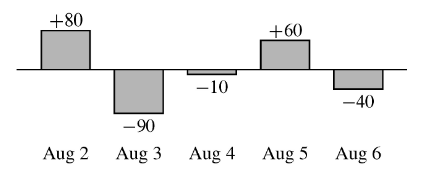
\includegraphics[height=0.2\textheight]{12.png}
\end{figure}

$80\times 5-90\times 4-10\times +60\times 2-40\times 1=90$, $90/6=15$, 故选E. 

13. Two transformations are said to commute if applying the first followed by the second gives the same result as applying the second followed by the first. Consider these four transformations of the coordinate plane:
\begin{enu} 
\item a translation 2 units to the right,
\item a $90^{\circ}$-rotation counterclockwise about the origin,
\item a reflection across the $x$-axis, and
\item a dilation centered at the origin with scale factor 2.
\end{enu}
Of the 6 pairs of distinct transformations from this list, how many commute?
(A) 1
(B) 2
(C) 3
(D) 4
(E) 5

(1)在复平面上为$z\mapsto z+2$, (2)为$\times i$, (3)为取共轭, (4)为$\times2$. 故可交换的有
$(1)(3)$, $(2)(4)$和 $(3)(4)$, 选C 

14. One side of an equilateral triangle of height 24 lies on line $\ell$. A circle of radius 12 is tangent to $\ell$ and is externally tangent to the triangle. The area of the region exterior to the triangle and the circle and bounded by the triangle, the circle, and line $\ell$ can be written as $a \sqrt{b}-c \pi$, where $a, b$, and $c$ are positive integers and $b$ is not divisible by the square of any prime. What is $a+b+c$ ?
(A) 72
(B) 73
(C) 74
(D) 75
(E) 76

$a=48,b=3,c=24$选D. 

15. Let $M$ be the greatest integer such that both $M+1213$ and $M+3773$ are perfect squares. What is the units digit of $M$ ?
(A) 1 (B) 2 (C) 3 (D) 6 (E) 8

$M=407108$, 选E. 

\begin{figure}[H]
    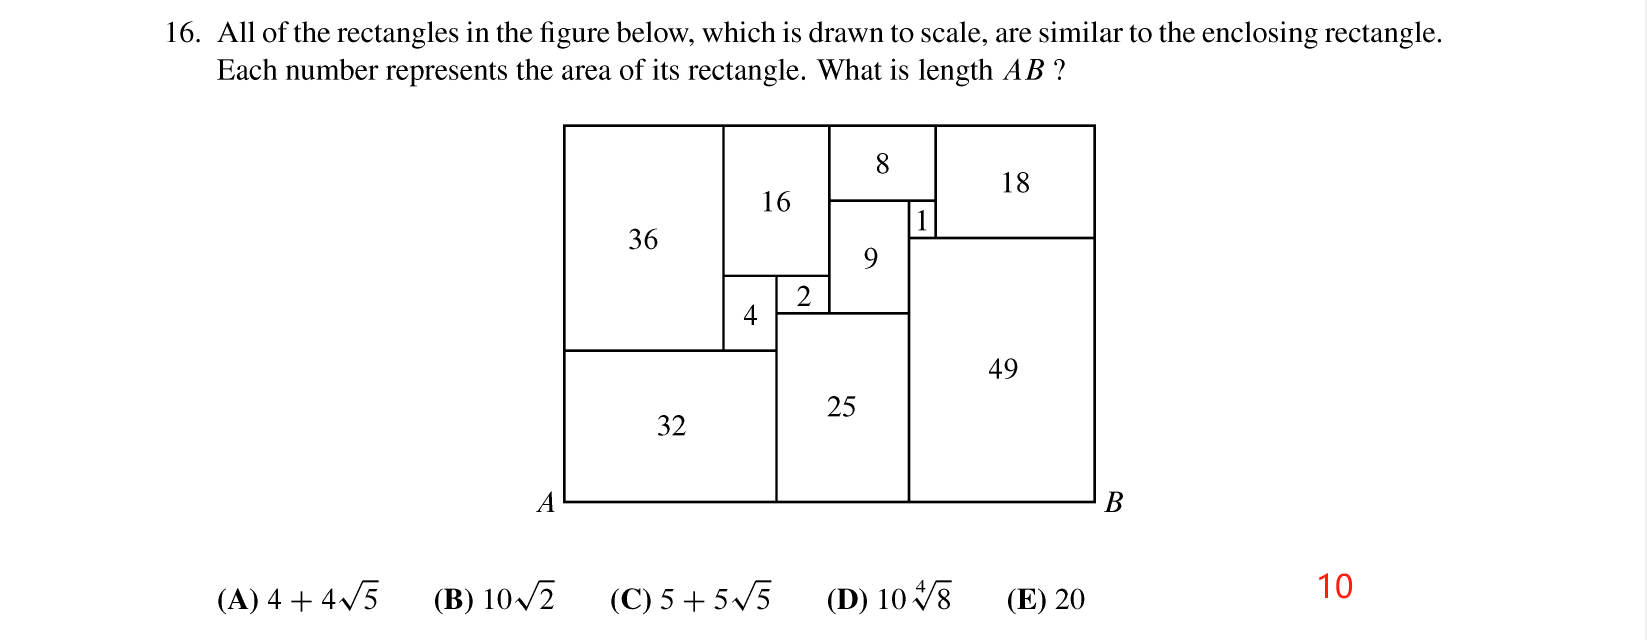
\includegraphics[height=0.3\textheight]{16.png}
\end{figure}
选D.


17. Two teams are in a best-two-out-of-three playoff: the teams will play at most 3 games, and the winner of the playoff is the first team to win 2 games. The first game is played on Team A's home field, and the remaining games are played on Team B's home field. Team A has a $\frac{2}{3}$ chance of winning at home, and its probability of winning when playing away from home is $p$. Outcomes of the games are independent. The probability that Team A wins the playoff is $\frac{1}{2}$. Then $p$ can be written in the form $\frac{1}{2}(m-\sqrt{n})$, where $m$ and $n$ are positive integers. What is $m+n$ ?
(A) 10
(B) 11
(C) 12
(D) 13
(E) 14

$m=4,n=10$选14. 

18. There are exactly $K$ positive integers $b$ with $5 \leq b \leq 2024$ such that the base- $b$ integer $2024_b$ is divisible by 16 (where 16 is in base ten). What is the sum of the digits of $K$ ?
(A) 16
(B) 17
(C) 18
(D) 20
(E) 21

$b\equiv 3,6,7\mod{8}$时满足条件, $K=758$, 选D. 

19. 19. The first three terms of a geometric sequence are the integers $a$, 720, and $b$, where $a<720<b$. What is the sum of the digits of the least possible value of $b$ ?
(A) 9
(B) 12
(C) 16
(D) 18
(E) 21

Python跑出来结果为$a=675, b=768$, 选E. 

20. Let $S$ be a subset of $\{1,2,3, \ldots, 2024\}$ such that the following two conditions hold:
\begin{enu} 
\item If $x$ and $y$ are distinct elements of $S$, then $|x-y|>2$.
\item If $x$ and $y$ are distinct odd elements of $S$, then $|x-y|>6$.
\end{enu}
What is the maximum possible number of elements in $S$ ?
(A) 436
(B) 506
(C) 608
(D) 654
(E) 675

考虑$\bbrace{1,4,8,11,14,18,21,24,28,31,34,38,\dots}$
选C.

21. The numbers, in order, of each row and the numbers, in order, of each column of a $5 \times 5$ array of integers form an arithmetic progression of length 5 . The numbers in positions $(5,5),(2,4),(4,3)$, and $(3,1)$ are $0,48,16$, and 12 , respectively. What number is in position $(1,2) ?$

$$
\left[\begin{array}{ccccc}
. & ? & \cdot & . & . \\
. & \cdot & \cdot & 48 & \cdot \\
12 & \cdot & \cdot & \cdot & \cdot \\
\cdot & \cdot & 16 & \cdot & . \\
\cdot & \cdot & . & . & 0
\end{array}\right]
$$
(A) 19
(B) 24
(C) 29
(D) 34
(E) 39

设$(1,1),(1,3),(2,1),(2,3)$分别为$12-2d,16-3t,12-d,16-2t$, 解得$d=0,t=-10$,故$(1,2)$为$29$,选C. 
 
\begin{figure}[H]
    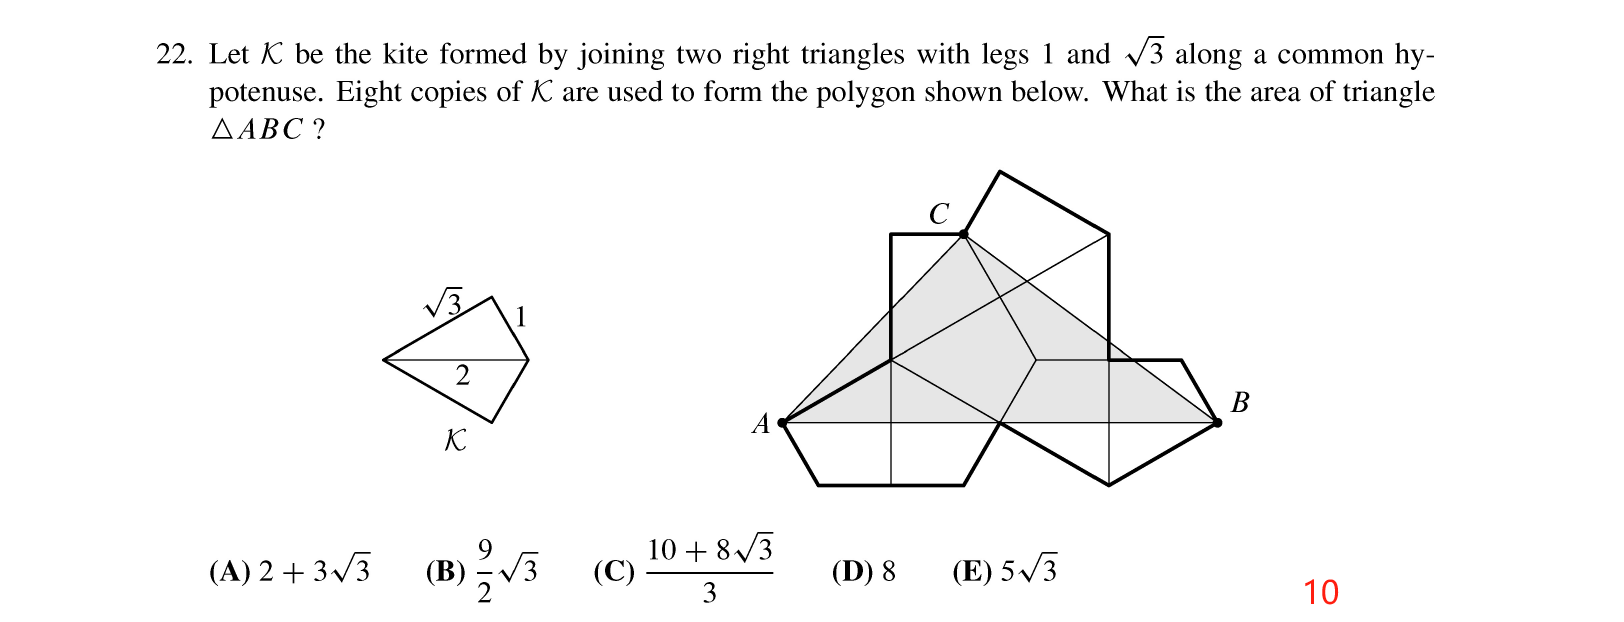
\includegraphics[height=0.3\textheight]{22.png}
\end{figure}

B 

23. Integers $a, b$, and $c$ satisfy $a b+c=100, b c+a=87$, and $c a+b=60$. What is $a b+b c+c a$ ?
(A) 212
(B) 247
(C) 258
(D) 276
(E) 284

$a=-9,b=-12,c=-8$选D.

\begin{figure}[H]
    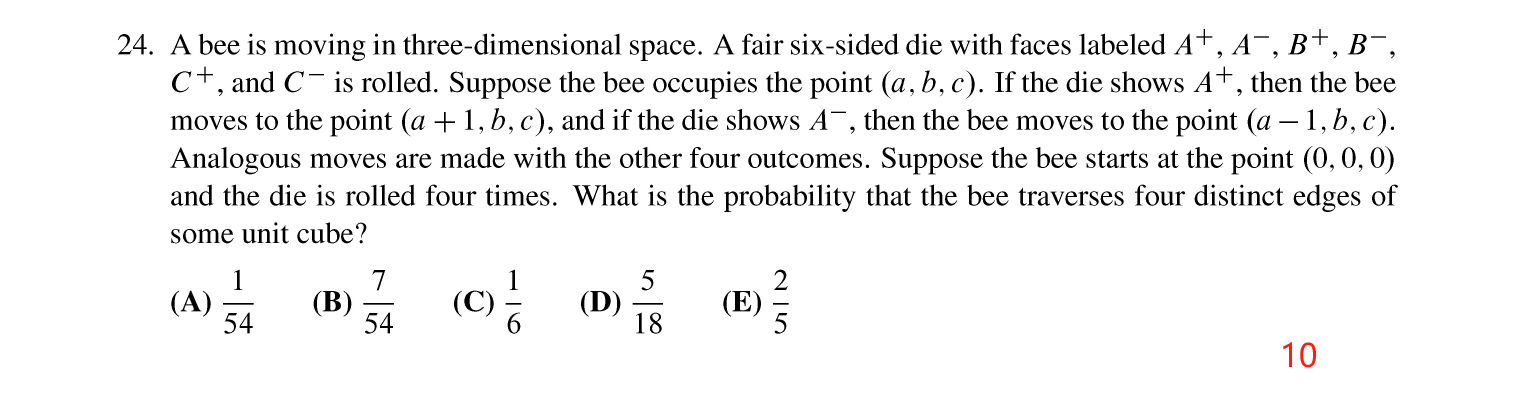
\includegraphics[height=0.2\textheight]{24.png}
\end{figure}
\begin{equation*}
   \frac{2}{3}\times (\frac{1}{6}\times \frac{1}{2}+ \frac{1}{3}\times \frac{1}{3})=\frac{7}{54}
\end{equation*}
选B. 

\begin{figure}[H]
    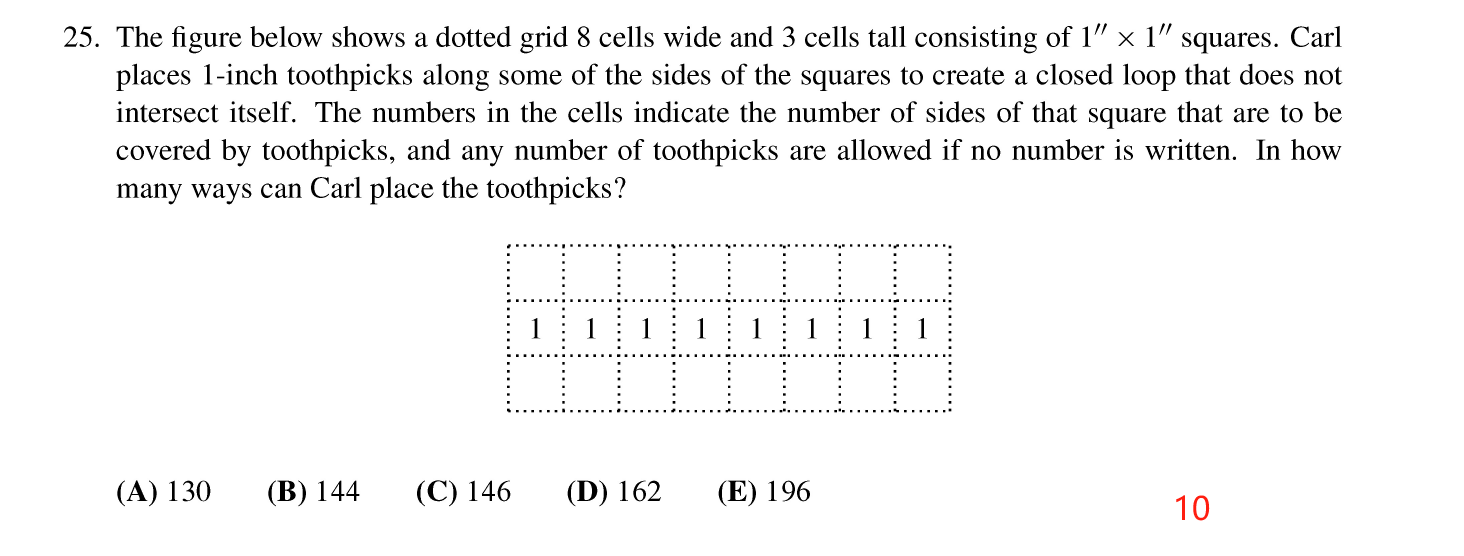
\includegraphics[height=0.3\textheight]{25.png}
\end{figure}
$2^6+2^5\times 4+ 2^4+ 2=146$选C. 













\end{document}